\documentclass{beamer}

% Theme choice
\usetheme{CambridgeUS} % professional, clean look
\usecolortheme{default} % colors can be adjusted if desired

% Packages
\usepackage[utf8]{inputenc}
\usepackage{graphicx}   % for including graphics
\usepackage{booktabs}   % for tables
\usepackage{amsmath, amssymb} % for math
\usepackage{hyperref}   % for clickable links

% Title page info
\title[Mobility Decisions Later in Life]{Wages vs Amenities}
\author[Tate Mason]{Tate Mason \\ \smallskip \texttt{Tate.Mason@uga.edu}}
\institute[Univ. of Georgia]{John Munro Godfrey Sr. Department of Economics \\ The University of Georgia}
\date{\today} % or custom date

% Begin document
\begin{document}

% Title page
\begin{frame}
  \titlepage
\end{frame}

% Outline
\begin{frame}{Outline}
  \tableofcontents
\end{frame}

\section{Introduction}
\begin{frame}{Motivation}
  \begin{itemize}
    \item Typically, location choice models focus on wages.
    \item Do other factors play a role in location decisions later in life?
    \item \textbf{Main Question:} How does motivation for moving change with age?
  \end{itemize}
\end{frame}

\section{Data}
\begin{frame}{Data Source}
  \begin{itemize}
    \item IPUMS USA data from 1990 - 2019
    \item Decennial censuses and ACS data
    \item Panel structure by linking individuals across years
  \end{itemize}
\end{frame}

\begin{frame}{Sample Selection}
  \begin{itemize}
    \item Individuals aged 40-85 at time of first observation
    \item Moved at least once during observation period
    \item Exclude group quarters, military, and missing data
    \item Final sample size: ~1.25 million households
  \end{itemize}
\end{frame}

\section{Empirical Facts}
\begin{frame}{Empirical Motivation}
  \begin{itemize}
    \item Younger movers and older movers exhibit different mobility patterns
    \item High income individuals move more with higher frequency
    \item Those without children move more often
    \item Probability of moving peaks at the age around retirement, and then declines
  \end{itemize}
\end{frame}

\begin{frame}{Summary Statistics}
  \begin{table}[htbp]
  \centering
  \caption{Summary Statistics: Movers vs.\ Non-Movers}
  \label{tab:movers_nonmovers}
    \begin{tabular}{lcc}
      \hline\hline
      & \textbf{Movers} & \textbf{Non-Movers} \\
      \hline
      N (households) & 185{,}813 & 940{,}861 \\
      \% own home & 42.4\% & 37.6\% \\
      \% married & 51.2\% & 38.4\% \\
      Avg.\ household income (\$) & 54{,}230.81 & 42{,}473.42 \\
      Avg.\ rent (renters / non-missing, \$) & 595.87 & 574.68 \\
      Avg.\ home value (owners / non-missing, \$) & 290{,}351 & 270{,}827 \\
      \hline
    \end{tabular}
  \end{table}
\end{frame}

\begin{frame}{Graphical Evidence}
  \begin{figure}
    \centering
    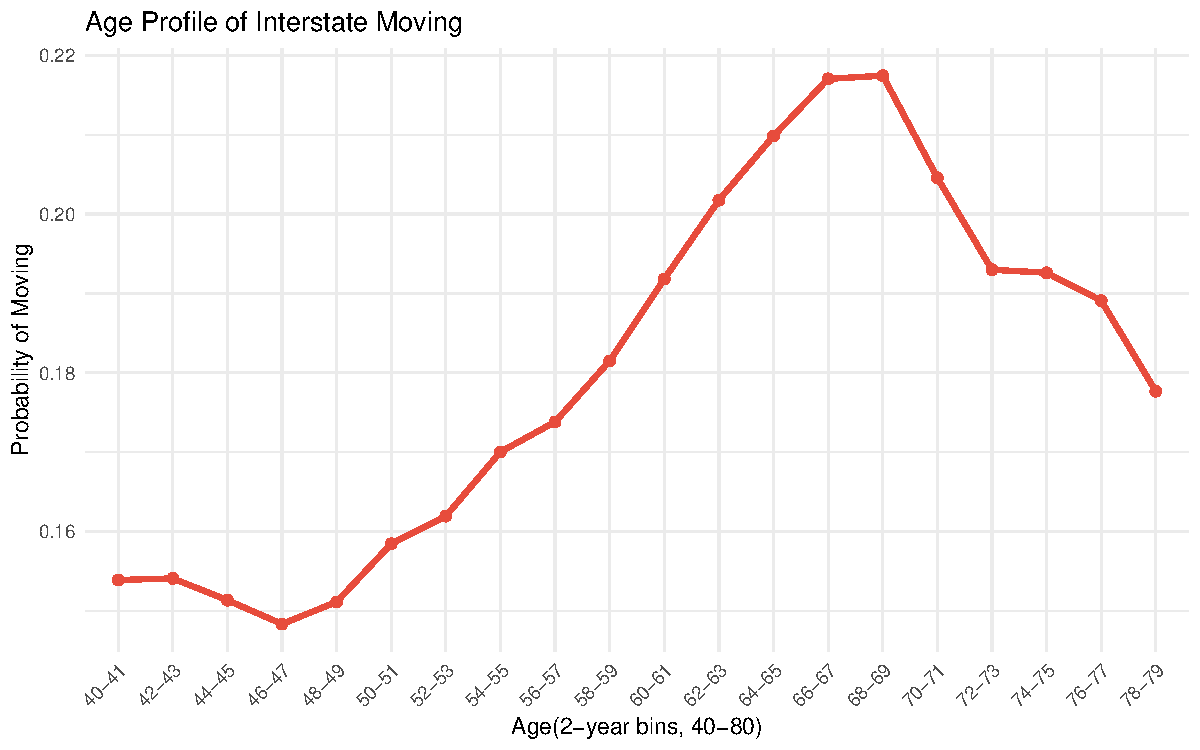
\includegraphics[width=0.8\linewidth]{figures/age_profile_move.pdf}
    \caption{Age Profile of Moving Frequency}
  \end{figure}
\end{frame}
\begin{frame}{Graphical Evidence}
  \begin{figure}
    \centering
    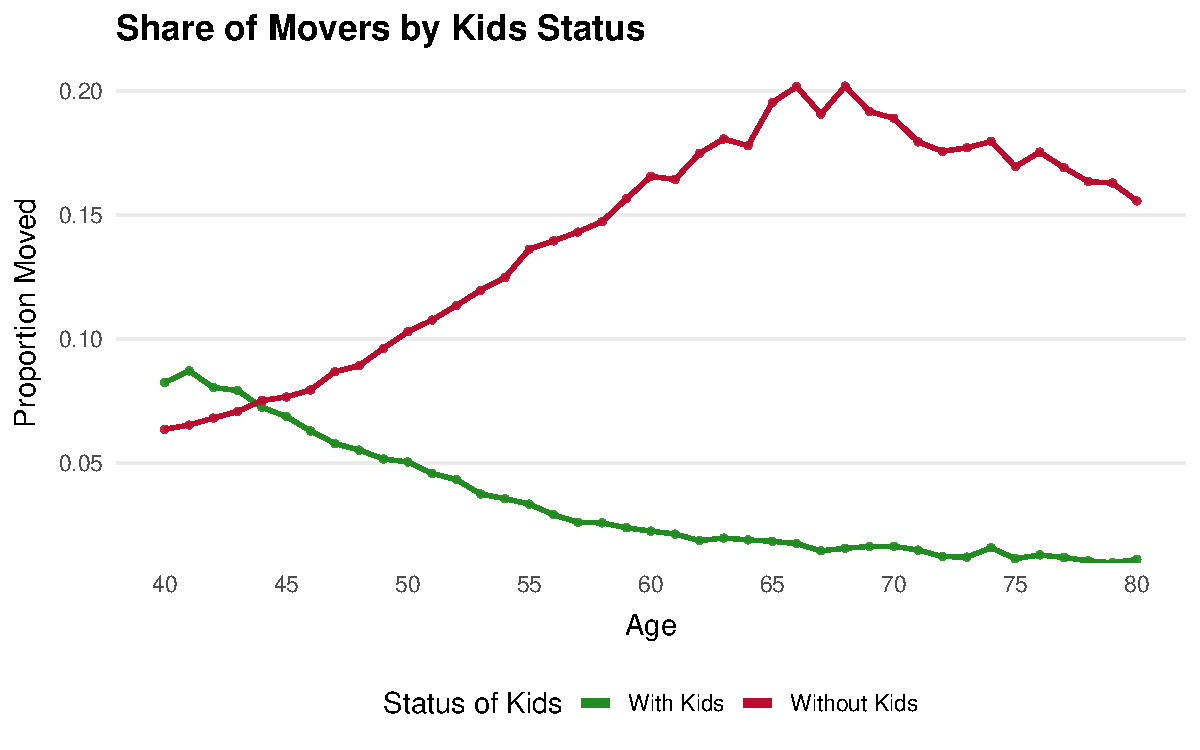
\includegraphics[width=0.8\linewidth]{figures/mover_prop_kids.pdf}
    \caption{Children vs No Children Moving Frequency}
  \end{figure}
\end{frame}
\begin{frame}{Graphical Evidence}
  \begin{figure}
    \centering
    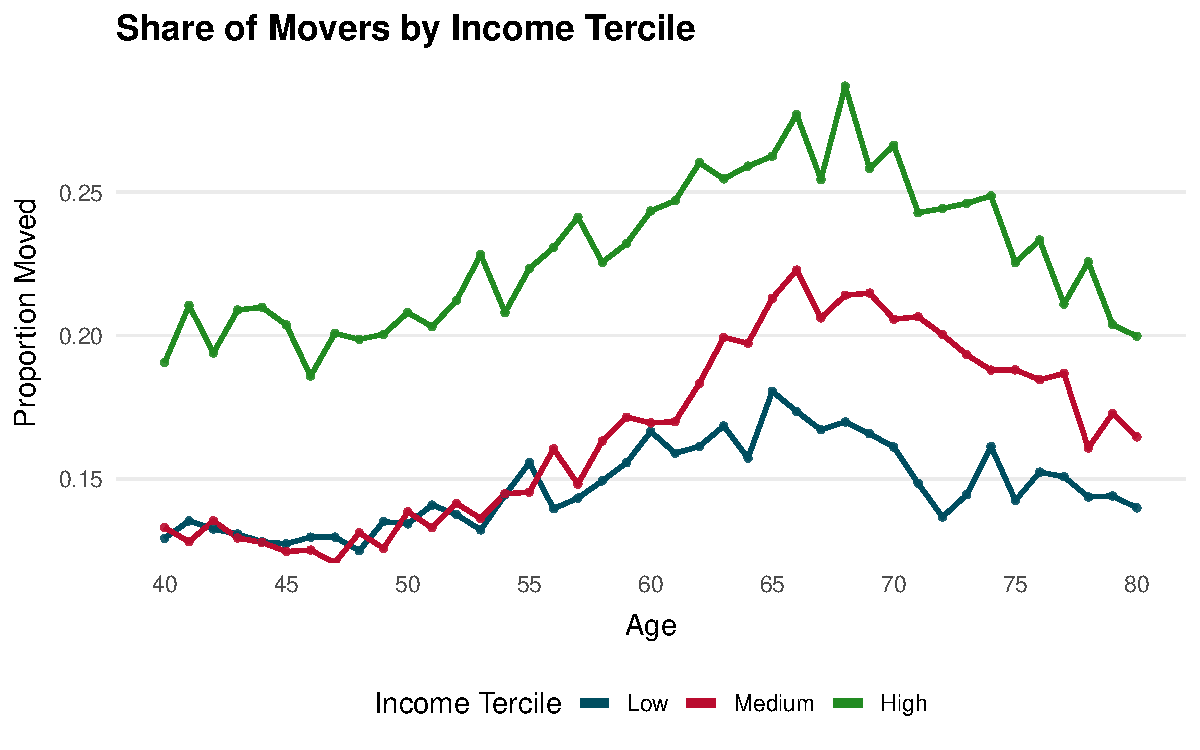
\includegraphics[width=0.8\linewidth]{figures/mover_prop_income.pdf}
    \caption{Income vs Moving Frequency}
  \end{figure}
\end{frame}
\begin{frame}{Graphical Evidence}
  \begin{figure}
    \centering
    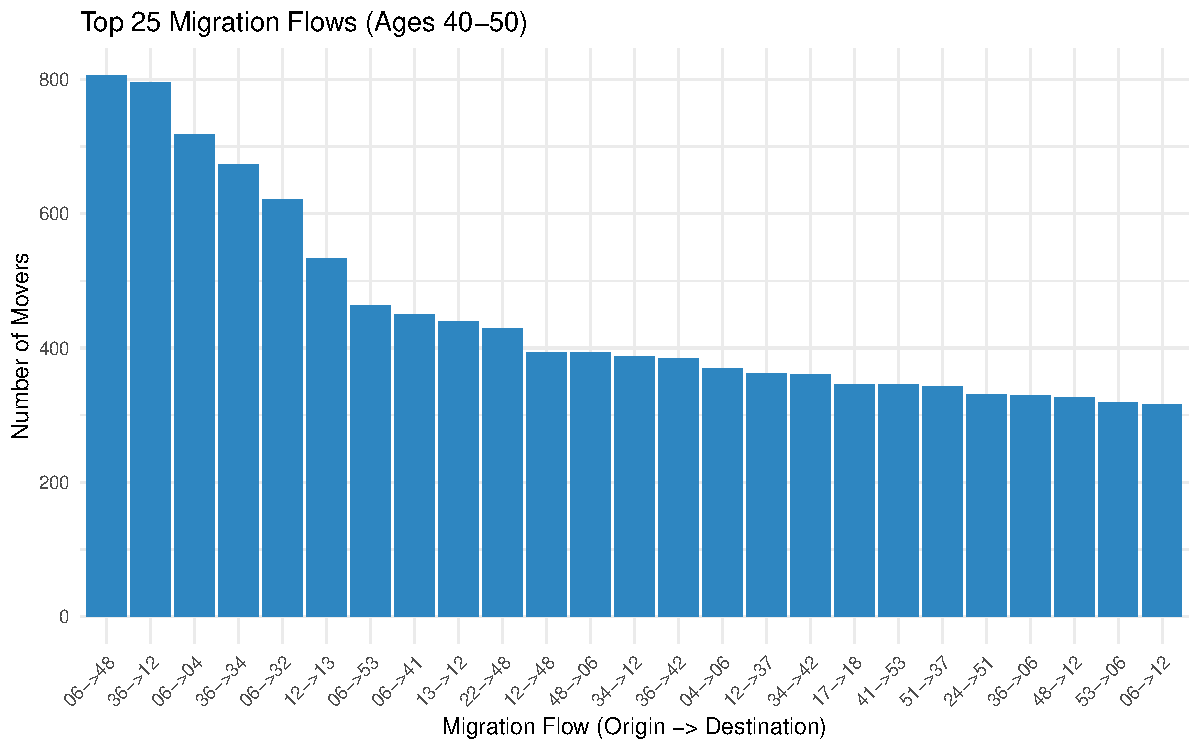
\includegraphics[width=0.8\linewidth]{figures/migration_flows_40_50.pdf}
    \caption{Migration Flows (Age 40-50)}
  \end{figure}
\end{frame}
\begin{frame}{Graphical Evidence}
  \begin{figure}
    \centering
    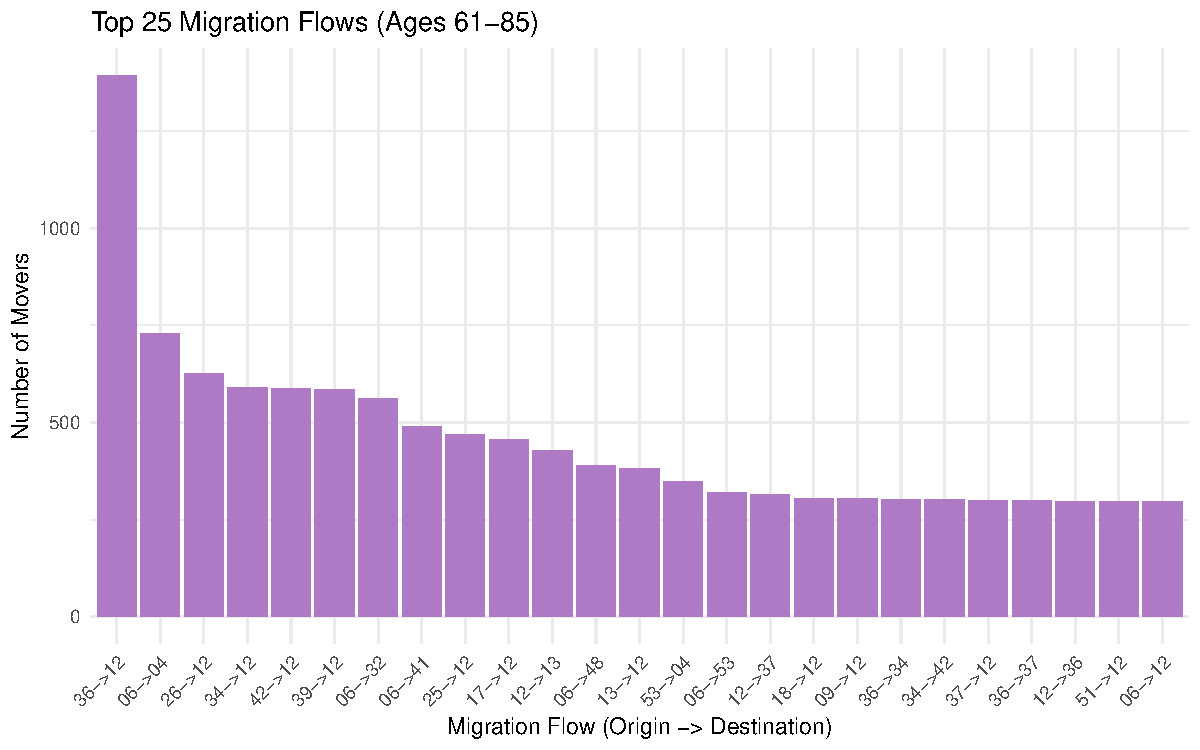
\includegraphics[width=0.8\linewidth]{figures/migration_flows_61_85.pdf}
    \caption{Migration Flows (Age 61-85)}
  \end{figure}
\end{frame}
\section{Model}
\begin{frame}{Model Overview}
  \begin{itemize}
    \item Two types: Workers, Retirees
    \item Workers supply labor inelastically, earn wages based on location, retire with probability $1-x$ each period
    \item Retirees receive pension income, base moving decisions on amenities, die with probability $1-y$ each period, replaced by new workers
    \item Both types maximize lifetime utility over consumption and amenities
  \end{itemize}
\end{frame}
\begin{frame}{Utility Function}
  \begin{itemize}
    \item Workers: $U^w(c, m(z);t) = \frac{-(c-\bar{c})^2}{2} - \gamma\cdot\{z'\ne z\}$
    \item Retirees: $U^r(c, m(z);t) = \frac{-(c-\bar{c})^2}{2} - \gamma\cdot\{z'\ne z\}$
    \item $c$: consumption, $m(z)$: amenities in location $z$
    \item $h(z)$: housing quality for workers, $hc(z)$: health care quality for retirees
    \item $\gamma$: moving cost parameter
  \end{itemize}
\end{frame}
\begin{frame}{Budget Constraints}
  \begin{itemize}
    \item Workers: $c_t = w(z_t) - \tau(z_t) - \mathbb{E}[c(h(z))|\delta]$
    \item $\delta$: Prior assumptions about housing costs in location $z'$
    \item $w(z_t)$: wage in location $z_t$, $\tau(z_t)$: taxes, $c(h(z))$: housing cost
    \item Retirees: $c_t + s_{t+1} = (1 + r)s_t + p - \mathbb{E}[c(hc(z))|\delta]$
    \item $p$: pension income
  \end{itemize}
\end{frame}
\begin{frame}{Decision Problem: Workers}
  \begin{equation}
    $V^w(\delta, z_t, t) = \max\{V_w^M(\delta, z_t, t), V_w^S(\delta, z_t, t)\}$
  \end{equation}
  \begin{itemize}
    \item $V_w^M$: value of moving, $V_w^S$: value of staying
  \end{itemize}
  \begin{equation}
    \item $V^S_w(\delta, z_t, t) = \max_{c_t} \{U(c_t) + x\beta V^w(\delta, z_t, t+1) + (1-x)\betaV^r(\delta,z_t, t+1)\}$
  \end{equation}
  \begin{equation}
    \item $V^M_w(s_t, z_t; t) = \max_{z', c_t} \{U(c_t, m(z')) + x\beta \mathbb{E}[V^w(\delta', z'; t+1)|\delta] + (1-x)\beta\mathbb{E}[V^r(\delta', z'; t+1)|\delta]\}$
  \end{equation}
\end{frame}
\begin{frame}{Decision Problem, Retirees}
  \begin{equation}
    $V^r(\delta, z_t; t) = \max\{V_r^M(\delta, z_t; t), V_r^S(z_t; t)\}$
  \end{equation}
  \begin{itemize}
    \item $V_r^M$: value of moving, $V_r^S$: value of staying
  \end{itemize}
  \begin{equation}
    \item $V^S_r(z_t; t) = \max_{c_t} \{U(c_t, m(z_t)) + y\beta V^r(\delta, z_t; t+1)\}$
  \end{equation}
  \begin{equation}
    \item $V^M_r(\delta, z_t; t) = \max_{z', c_t} \{U(c_t, m(z')) + y\beta V^r(\delta', z'; t+1)\}$
  \end{equation}
\end{frame}
\section{Next Steps}
\begin{frame}{Next Steps}
  \begin{itemize}
    \item Find a suitable measure of quality of life for locations
    \begin{itemize}
      \item Health care quality
      \item Climate
      \item Cost of Living
    \end{itemize}
    \item Calibrate model parameters using observed mobility patterns
  \end{itemize}
\end{frame}
\begin{frame}{Thank You}
  \begin{center}
    \Huge Thank You! \\
    \vspace{1cm}
    \Large Questions?
  \end{center}
\end{frame}

\end{document}
